\section{Evaluation}\label{sec-eval}

In this section we evaluate the effectiveness of Sensibility Testbed's 
privacy mechanisms, its usability as a mobile testbed, and its 
performance. To investigate whether the policies provided by 
Sensibility Testbed are representative, we surveyed the projects
in the past few years and identified their security and privacy 
mechanisms. We analyzed if Sensibility Testbed can provide policies 
to protect the corresponding data in Section~\ref{sec-our-policies}. 
We then show two examples by applying Sensibility Testbed's 
policies to two experiments in Section~\ref{sec-experiment}. We 
demonstrate that with the policies in place, we can protect the 
device owner's privacy, while the data is sufficient for answering 
research questions. We show the performance overhead of 
Sensibility Testbed in Section~\ref{sec-benchmark}, and our 
deployment experience in Section~\ref{sec-deployment}.

%\todo{Q: how well the testbed protects privacy, and still allows experiments
%to function? A: \ref{sec-accurate} and \ref{sec-function}.}


\subsection{Sensibility Testbed's Privacy Policies}\label{sec-our-policies}

\begin{table}
\scriptsize
\centering

\bgroup
\def\arraystretch{1.15}% % for table padding
\begin{tabular}{|l|l|c|c|c|}
\hline
\multirow{2}{.8cm}{\bf Project} & \multirow{2}{*}{\bf Sensor} & 
\multicolumn{3}{c|}{\bf Equivalent Sensibility Testbed policy} \\\cline{3-5}
& & {\bf Default} & {\bf Specialized} & {\bf N/A} \\\hline

EnCore~\cite{aditya2014encore}  & Bluetooth & \tickmark &   &   \\\hline

\multirow{2}{*}{\cite{chen2014sensor}\textsuperscript{*}} & Accelerometer 
& \tickmark &   &  \\ \cline{2-5}
& Camera & & \tickmark & \\ \hline

\multirow{5}{.8cm}{ProtectMyPrivacy \cite{agarwal2013protectmyprivacy}} & Device ID & & \tickmark & \\ \cline{2-5}
& WiFi & \tickmark &   &  \\ \cline{2-5}
& Bluetooth & \tickmark &   & \\ \cline{2-5}
& Address book & & \tickmark & \\ \cline{2-5}
& Location & \tickmark &   &   \\\hline
 
\multirow{4}{*}{CQue~\cite{parate2013leveraging}}  & Location & \tickmark &  & \\\cline{2-5}
& Accelerometer & \tickmark &   &  \\ \cline{2-5}
& Gyroscope & \tickmark &   &  \\ \cline{2-5}
& Bluetooth & \tickmark &   &   \\\hline

\multirow{2}{*}{MaskIt~\cite{gotz2012maskit}} & Location & \tickmark &   & \\\cline{2-5}
& Cellular & \tickmark &   &   \\\hline

\multirow{3}{*}{Jigsaw~\cite{lu2010jigsaw}} & Accelerometer 
& \tickmark &   &  \\ \cline{2-5}  
& Microphone  & & \tickmark & \\ \cline{2-5}
& Location & \tickmark &   &   \\\hline

Cach{\'e}~\cite{amini2011cache} & Location & \tickmark &   &   \\\hline

\cite{jiang2012isolating}\textsuperscript{*} & Cellular & \tickmark &   &   \\\hline

\multirow{2}{*}{TapPrints~\cite{miluzzo2012tapprints}} & Accelerometer 
& \tickmark &   &  \\ \cline{2-5}  
& Gyroscope & \tickmark &   &  \\ \hline

\multirow{4}{.8cm}{FindingMiMo \cite{shin2011findingmimo}} 
& WiFi & \tickmark &   &  \\ \cline{2-5}
& Location & \tickmark &  & \\\cline{2-5}
& Accelerometer & \tickmark &   &  \\ \cline{2-5}
& Magnetometer & \tickmark &   &  \\ \hline

ACCessory~\cite{owusu2012accessory} & Accelerometer & \tickmark &   
&  \\ \hline

TouchLogger~\cite{cai2011touchlogger} & Gyroscope & \tickmark &   
&  \\ \hline

\multirow{6}{*}{MockDroid~\cite{beresford2011mockdroid}} 
& Location & \tickmark &  & \\\cline{2-5}
& Internet\textsuperscript{\dag} & \tickmark & & \\ \cline{2-5}
& Cellular & \tickmark &   &  \\ \cline{2-5}
& Address book & & \tickmark & \\ \cline{2-5}
& Device ID & & \tickmark & \\ \cline{2-5}
& Broadcast intent & \tickmark &   &  \\ \hline

\multirow{6}{*}{Guardian \cite{zhang2015leave}} 
& Bluetooth & \tickmark &   & \\ \cline{2-5}
& Internet\textsuperscript{\dag} & \tickmark & & \\ \cline{2-5}
& Microphone  & & \tickmark & \\ \cline{2-5}
& Cellular & \tickmark &   &  \\ \cline{2-5}
& Motion sensors & \tickmark &   &  \\ \cline{2-5}
& CPU usage\textsuperscript{\ddag} & \tickmark & & \\\hline

\cite{aviv2012practicality}\textsuperscript{*} & Accelerometer & \tickmark &   
&  \\ \hline

\multirow{2}{*}{\cite{cai2012practicality}\textsuperscript{*}} & Accelerometer 
& \tickmark &  &  \\ \cline{2-5}
& Gyroscope & \tickmark & &  \\ \hline

AccelPrint~\cite{dey2014accelprint} & Accelerometer & \tickmark &   
&  \\ \hline

\multirow{8}{*}{\cite{bojinov2014mobile}\textsuperscript{*}} & Microphone  
& & \tickmark & \\ \cline{2-5}
& Accelerometer & \tickmark &   &  \\ \cline{2-5}
& Gyroscope & \tickmark & &  \\ \cline{2-5}
& Magnetometer & \tickmark &   &  \\ \cline{2-5}
& Ambient light & \tickmark &   &  \\ \cline{2-5}
& Location (GPS) & \tickmark &   &  \\ \cline{2-5}
& Touch screen & & & \xmark \\ \cline{2-5}
& Camera & & \tickmark & \\ \hline

Gyrophone~\cite{michalevsky2014gyrophone} & Gyroscope 
& \tickmark & &  \\ \hline

\cite{shokri2011quantifying}\textsuperscript{*}
& Location & \tickmark &   &  \\ \hline

\cite{polakis2015s}\textsuperscript{*}
& Location & \tickmark &   &  \\ \hline

AnonySense~\cite{kapadia2008anonysense} 
& Location & \tickmark &   &  \\ \hline

\cite{liu2015good}\textsuperscript{*} 
& Accelerometer & \tickmark &   &  \\ \hline

LP-Guardian~\cite{fawaz2014location} 
& Location & \tickmark &   &  \\ \hline

\cite{bordenabe2014optimal}\textsuperscript{*}
& Location & \tickmark &   &  \\ \hline

PrivStats~\cite{popa2011privacy}
& Location & \tickmark &   &  \\ \hline

\multirow{5}{*}{ipShield~\cite{chakraborty2014ipshield}} 
& Location (GPS) & \tickmark &   &  \\ \cline{2-5}
& Accelerometer & \tickmark &   &  \\ \cline{2-5}
& Gyroscope & \tickmark & &  \\ \cline{2-5}
& WiFi & \tickmark &   &  \\ \cline{2-5}
& Cellular & \tickmark &   & \\ \hline
 
\multirow{3}{*}{TaintDroid~\cite{enck2014taintdroid}} & Location & \tickmark &   &  \\ \cline{2-5}
& Accelerometer & \tickmark &   &  \\ \cline{2-5}
& Internet\textsuperscript{\dag} & \tickmark & & \\ \hline

\multicolumn{5}{l}{\textsuperscript{*}\scriptsize These projects do not have a project name.} \\ 

\multicolumn{5}{l}{\textsuperscript{\dag}\scriptsize Internet connectivity policies
can be implemented by interposing socket calls.} \\

\multicolumn{5}{l}{\textsuperscript{\ddag}\scriptsize CPU usage can be obtained
through reading the files in \path{/proc/stat}.} \\

\end{tabular}
\egroup

\caption{\small Sensibility Testbed's support for privacy and security policies. A default 
policy is supported by Sensibility Testbed without extra effort. A specialized policy can 
be supported by extending default policies. A policy is marked as N/A if it is not possible 
to provide support.}
\label{tab:policy}
%\vspace{-10pt}
\end{table}

%\todo{Q1: does ST protect privacy sufficiently?}

\begin{table}
\scriptsize
\centering

\bgroup
\def\arraystretch{1.15}% % for table padding
\begin{tabular}{|l|l|c|c|c|}
\hline
\multirow{2}{.8cm}{\bf Project} & \multirow{2}{*}{\bf Sensor} & 
\multicolumn{3}{c|}{\bf Equivalent Sensibility Testbed policy} \\\cline{3-5}
& & {\bf Default} & {\bf Specialized} & {\bf N/A} \\\hline

Koi~\cite{guha2012koi} & Location & \tickmark &   &  \\ \hline

Locaccino~\cite{toch2010empirical} & Location & \tickmark &   &  \\ \hline

\multirow{2}{*}{Accomplice~\cite{han2012accomplice}} & Location & \tickmark &   &  \\ \cline{2-5}
& Accelerometer & \tickmark &   &  \\ \hline

\multirow{2}{*}{\bf Total} & \multirow{2}{*}{\bf 71} & \multirow{2}{1cm}{\bf 
61/71 (85.92\%)} & \multirow{2}{1cm}{\bf 9/71 (12.67\%)} & 
\multirow{2}{1cm}{\bf 1/71 (1.41\%)} \\ & & & & \\\hline

\end{tabular}
\egroup

\caption{\small Table~\ref{tab:policy} continued --- Sensibility Testbed's support 
for privacy and security policies. }
\label{tab:policy-continued}
%\vspace{-10pt}
\end{table}


\textbf{Privacy and security concerns.}
In order to identify the current privacy and security concerns on mobile 
devices, we surveyed 31 projects in the past few years. We then analyzed
these projects by reading their corresponding publications, identified 
their needs or their provided mechanism for privacy protection. 
These projects, listed in Table~\ref{tab:policy} and \ref{tab:policy-continued},
range from social network applications~\cite{aditya2014encore} to facial
recognition algorithms~\cite{chen2014sensor}. If their privacy need or privacy
protection can be supported by equivalent \textit{default} policies in Sensibility 
Testbed, a \tickmark\ is marked in the default column. These sensors belong to 
low to moderate risk, as defined in Table~\ref{tab:default}. Similarly, if the
sensors are of high risk, a \tickmark\ is marked in the specialized column. 
This means that a different IRB procedure could be followed to extend 
default policies (Section~\ref{sec-irb-policies}). If a sensor cannot be 
supported by a default or specialized policy, a \xmark\ is marked in the 
N/A column. 

Out of these projects, 
19 of them proposed privacy protection about location information, 16 of 
them considered motion sensors such as accelerometer and gyroscope 
risky, and 9 had concerns about wireless network such as WiFi and Bluetooth
(connection/pairing history, MAC addresses, etc.). As expected, location (mainly GPS)
and motion sensors (mainly accelerometer) have the most privacy and security 
concerns~\cite{chakraborty2014ipshield}.
%\todo{Q1.1: what privacy concerns do people have? }

\textbf{Are Sensibility Testbed's policies sufficient?}
As shown in Table~\ref{tab:policy} and \ref{tab:policy-continued}, nearly 86\% 
of the security and privacy issues in prior projects can be addressed in 
Sensibility Testbed using default policies, and 13\% issues can be resolved by extending 
default policies (specialized policies). Only about 1\% of them cannot
be protected by the policies in Sensibility Testbed, \yanyan{I'm not sure 
yet how to explain this. I don't know what experiment would need this.}

In particular, prior work shows 
that Android users' touch inputs can be revealed through a few attack 
techniques like keyloggers and fingerprinting. 
%For example, a smartphone's accelerometer 
%and gyroscope can disclose shift and rotation data when a user types 
%through a software keyboard. Imprecisions in sensor calibration can 
%result in a device-specific scaling and thus can be a reliable fingerprint 
%of the device. 
User generated data thus can be informative enough 
for malware to infer the key the user enters~\cite{cai2011touchlogger, 
owusu2012accessory}, or to fingerprint and identify individual 
devices~\cite{bojinov2014mobile, dey2014accelprint}. Because these 
motion sensors are accessible 
%through JavaScript in a mobile web browser, 
without requesting any 
permissions or notifying the device owner, these attack techniques are much 
less detectable. However, the chance for these techniques to succeed
depends on their sampling rate. 
%Consider an Android 
%user's average typing speed of 3 keys per second, when the sampling 
%rate goes down to once per second, the best the adversary can do is 
%just to identify 1 of these 3 keys. 
Therefore, the policies to restrict the access rates to motion sensors 
are effective when the allowed rate is lower than the best keylogger 
would require to identify a key, or the best tracker to fingerprint a device.
Section~\ref{sec-experiment} shows such an example. 

Another line of attack is on location privacy. \yanyan{need to wirte more here.
should we do an experiment for location?}

%\todo{Q1.2: does ST address these concerns? A1.2: show
%  a handful of past experiments with a 90/10 rule -- 90\% of experiments
%  can be doone with virtually no mods, and the other 8\% we can write 
%  specialized policy for and 2\% it's too hard.}

\subsection{Privacy Protection and Experiment Functionality}\label{sec-experiment}

\todo{Q2: is ST useful for answering research questions? A:
compare the results of an algorithm with varying levels of 
data precision (Seth's algorithm?), and show a diagram suggested
by Justin.}

\yanyan{with the privacy protection in place, is the data we 
provide sufficient for experiments to function?}

%\subsection{Usability}\label{sec-usability}
%
%\yanyan{user survey on privacy: show how people feel if their 
%privacy has been protected, whether device owners feel the 
%protection is enough.}
%
%\yanyan{incentives to participants}

\subsection{Microbenchmarks}\label{sec-benchmark}

We measured the overhead incurred by running blurring layers with 
experiment code in Sensibility Testbed, to demonstrate that it is 
feasible to protect sensor data privacy on end-user devices without 
affecting user experience. 
%in terms of app responsiveness and battery life.

\begin{figure}
\center{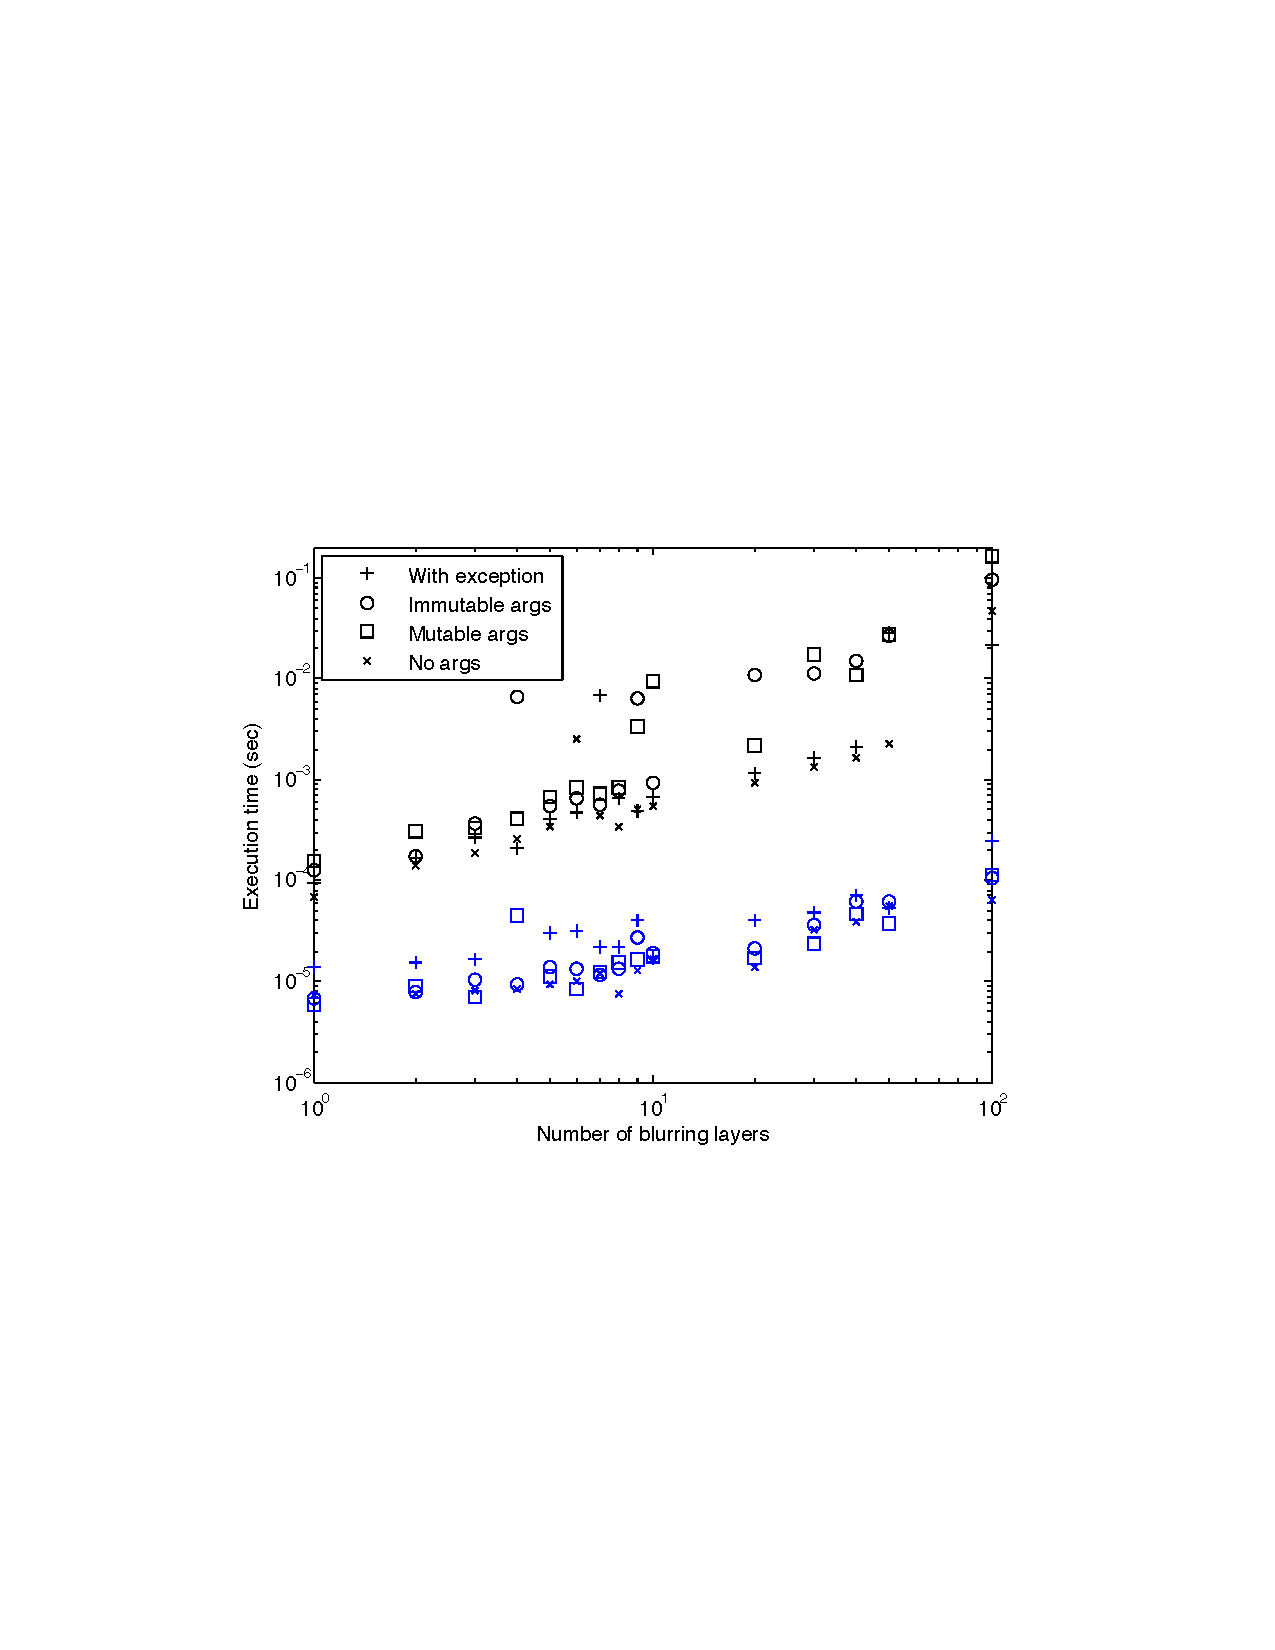
\includegraphics[width=3in]{figs/time.pdf}}
\caption{\small Overhead incurred by running varying number of blurring 
layers with experiment code. Blue points show the execution time of 
an experiment using blurring layers without verifying the runtime behavior. 
Black points show the execution time with the runtime behavior verified. 
\label{fig-time}}
\end{figure}

%\textbf{Runtime overhead.}
Figure~\ref{fig-time} shows the runtime overhead of using varying number of 
blurring layers, i.e., policies, to protect sensor data. The experiment code 
uses calls \path{get_battery()} in the Repy sandbox. Each point in the 
figure is averaged over 100 iterations. Blue points show the execution time of 
using blurring layers without verifying the runtime behavior. Black points 
show the execution time with the runtime behavior verified, i.e., using a 
contract to check arguments, return values and exceptions. Note that a 
contract checks for both mutable and immutable data types~\cite{muta} 
for arguments and return values. When the number of layers is below 10, 
the runtime is slightly increased from 10$^{-5} s$ to 10$^{-4} s$. Although
the runtime overhead is higher with more layers, as Table~\ref{tab:policy} 
and \ref{tab:policy-continued} show, most projects need less than 10
policies. 

Table~\ref{tab:overhead}(a) shows the total runtime overhead when an experiment
calls \path{get_accelerometer()}, without any blurring layer (no layer), with blurring 
layers but without verifying the runtime behavior (no-op), and with blurring layers
that verifies the runtime behavior and rounds up accelerometer to two decimal 
points (round-up). As shown in the table, the total runtime is \textit{linear} with an 
increasing number of layers/policies. The overhead per policy is almost
constant, with no-op round 0.12 - 0.14 $ms$ and round-up 0.14 - 0.21 $ms$. 
Therefore, the runtime overhead will not affect conducting an 
experiment or user experience.

Table~\ref{tab:overhead}(b) shows the memory overhead without any blurring layer 
(no layer), and with blurring layers that verifies the runtime behavior and rounds up 
decimal points (round-up). As the results show, the memory overhead is almost
constant, around 0.48 - 0.55 $MB$, until the number of blurring layers reaches 100. 
\yanyan{is there an explanation?} Nevertheless, the overhead never exceeded 1 
$MB$ in all cases. 

\begin{table}
\scriptsize
\centering

\bgroup
\def\arraystretch{1.15}% % for table padding

\begin{tabular}{|l|l|c|c|c|c|}
\hline
\multicolumn{2}{|c|}{\multirow{2}{*}{\bf Operations}} & 
\multicolumn{4}{c|}{\bf Number of blurring layers} \\\cline{3-6}
\multicolumn{2}{|c|}{} & {\bf 3} & {\bf 10} & {\bf 50} & {\bf 100}\\\hline

\multicolumn{2}{|c|}{No layer (baseline)} & \multicolumn{4}{c|}{6.276 $ms$} \\\hline

\multirow{2}{*}{No-op} & Total & 6.654 $ms$ & 7.756 $ms$ & 12.75 $ms$ & 18.94 $ms$ \\ 
& Per-layer & 0.1259 $ms$ & 0.1479 $ms$ & 0.1295 $ms$ & 0.1266 $ms$ \\\hline

\multirow{2}{*}{Round-up} & Total & 6.907 $ms$ & 7.991 $ms$  & 13.86 $ms$ & 20.64 $ms$ \\ 
& Per-layer & 0.2104 $ms$ & 0.1715 $ms$ & 0.1518 $ms$ & 0.1436 $ms$ \\\hline 
\multicolumn{6}{c}{\vspace{-0.1cm}}\\

\multicolumn{6}{c}{\small (a) Runtime overhead.} \\
\end{tabular}\\\vspace{0.25cm}
%\end{subtable}


\begin{tabular}{|l|l|c|c|c|c|}
\hline
\multicolumn{2}{|c|}{\multirow{2}{*}{\bf Operations}} & 
\multicolumn{4}{c|}{\bf Number of blurring layers} \\\cline{3-6}
\multicolumn{2}{|c|}{} & {\bf 3} & {\bf 10} & {\bf 50} & {\bf 100}\\\hline

\multicolumn{2}{|c|}{No layer (baseline)} & \multicolumn{4}{c|}{6.246 $MB$} \\\hline

\multicolumn{2}{|c|}{Round-up} & 6.742 $MB$ & 6.801 $MB$ & 6.727 $MB$ & 7.230 $MB$ \\\hline

\multicolumn{2}{|c|}{Overhead} & 0.492 $MB$ & 0.555 $MB$ & 0.480 $MB$ & 0.984 $MB$ \\\hline
\multicolumn{6}{c}{\vspace{-0.1cm}}\\

\multicolumn{6}{c}{\small (b) Memory overhead.} \\
\end{tabular}
%\end{subtable}

\egroup

\caption{\small Overhead with varying number of blurring layers. }
\label{tab:overhead}
%\vspace{-10pt}
\end{table}


%\textbf{CPU and memory overhead.}
%\todo{what's the CPU/memory overhead?}

\subsection{Deployment Experience}\label{sec-deployment}

%\todo{Q3: how is the testbed being used? A: deployment experience: 
%number of people, projects, issues, hackathon.}

%\subsubsection{External Projects and Collaboration}\label{sec-external}

Sensibility Testbed has been adopted by projects such as 
Open3G~\cite{open3g} that investigates on cellular technologies 
and coverage, a vehicle data collection project~\cite{reininger2015first} 
that monitors vehicle traffic patterns. The experience from the 
project developers was positive, and they identified cases where our 
instructions for use were unclear. Despite these clarification issues, in 
the case of Open3G, the developer reported that writing the code to
get cellular information took about an hour and they have used our
testbed since 2012. We are currently in discussions with other 
researchers about integrating Sensibility Testbed into their research
projects, such as monitoring construction safety.

In 2014, we hosted a Hack-a-thon styled, one-day workshop co-located with 
the IEEE Sensors Applications Symposium (SAS) \cite{sas}. About twenty 
workshop participants with various backgrounds worked in teams 
for six hours and built four functional applications using Sensibility 
Testbed. None of the participants had any prior experience with 
this testbed, and many of them had no background in Computer
Science. With this success, we hosted a second workshop with 
SAS in 2015, and will continue in 2016. Interesting experiments 
developed by the participants include a device network monitor: 
when the battery level of a device is low, WiFi or Bluetooth that 
requires high power is turned off.

\textbf{Ease of use.}
%\label{sec-ease}
\todo{Q4: how easy is it to use the testbed? A: ease of use: 
compared to common measurement app (Android), 
how many lines of code can one save.}

\yanyan{how much time a student spent doing some
measurements (like Thomas's motion detection alg).}

\yanyan{compare to other projects,  developers can save
thousands of lines of code, and reuse the same set of 
devices.}
